\documentclass{article}
\usepackage[top=1in, bottom=1in, left=1in, right=1in]{geometry}
\usepackage{polski}
\usepackage[utf8]{inputenc}
\usepackage{graphicx}
\usepackage{hyperref}
\begin{document}
\title{\huge\bfseries Wyznaczanie przyspieszenia ziemskiego przy pomocy wahadła matematycznego}
\date{}
\maketitle
\section{Wstęp teoretyczny}
\subsection{Siła grawitacji}
Siła Grawitacji czyli siła ciążenia powszechnego jest zjawiskiem naturalnym, polegającym na oddziaływaniu na siebie, wzajemnie przyciągając się,  wszystkich obiektów które posiadają masę.\\\\
	Opierając sie na zależności siły grawitacyjnej, możemy obliczyć siłę $F_g$ z jaką planeta oddziałowuje na ciało o masie $m$:
	$$F_g = \frac{GM_zm}{{r_z^2}}$$
	 \begin{center}
	 $M_z \approx 5,9736 * 10^{24}$ kg - masa Ziemi, $r_z \approx 6373,14$km
	 \end{center}
\subsection{Przyspieszenie ziemskie, jednostka, zależność wartości od szerokości geograficznej i wysokości nad poziomem morza}
Przyspieszenie ziemskie - g jest to przyspieszenie grawitacyjne działająca na ciała swobodnie spadające na Ziemię(pomijając opory ruchów). 
$$g = \frac{GM_z}{r^2} \approx \frac{6,6732 \cdot 10^{-11} \cdot m^3\cdot kg^{-1}\cdot s-2 \cdot 5,9736 \cdot 10^{24}kg}{(6373,14km)^2} \approx 9,81 \frac{m}{s^2}$$
$$[g] = \frac{N}{kg} = \frac{m}{s^2}$$
Wartość przyspieszenia ziemskiego jest zależna od szerokości geograficznej oraz od wysokości nad poziomem morza. Przy wzroście wysokości, zwiększa się odległość od środka Ziemi, przez co przyspieszenie ziemskie maleje.\\
Wpływ na przyspieszenie ziemskie spowodowane szerokością geograficzną wynika z ruchu obrotowego Ziemi - na ciało znajdujące się na powierzchni planety działa siła odśrodkowa o przeciwnym zwrocie do siły grawitacji, przez co obserwujemy dany spadek wartości.
\subsection{Wahadło matematyczne oraz zależność okresu drgań od długości jego wahadła}
Idealnym wahadłem matematycznym możemy nazwać punktową masę m, zawieszoną na nieważkiej i nierozciągliwej linie. W praktyce, przybliżonym tworem jest niewielka metalowa kulka zawieszona na mocnej nitce. Okres drgań wahadła nie zależy od masy m tylko od długości wahadła l i dla małych kątów wynosi:
$$T = 2\pi \sqrt\frac{l}{g}$$
\begin{flushright}
\begin{scriptsize}
Źródła: \textit{http://www.fizykon.org/grawitacja/grawitacja$\_$wprowadzenie.htm} \\
\textit{http://pl.wikipedia.org/wiki/Grawitacja}\\
\textit{http://pl.wikipedia.org/wiki/Przyspieszenie$\_$ziemskie}\\
\end{scriptsize}
\end{flushright}
\section{Przebieg i cel ćwiczenia}
Celem tego ćwiczenia jest wyznaczenie przyspieszenia ziemskiego przy pomocy wahadła matematycznego. Na naszym stanowisku umieszczona jest urządzenie, składa się one z poprzeczki ze skalą milimetrową, na której jest zawieszone wahadło matematyczne. Długość wahadła można regulować. Urządzenie wyposażone jest w fotokomórkę, która mierzy czas N wahnięć ( w naszym przypadku N = 10 ). Na początku ćwiczenia ustalono długość wahadła (L = 20 cm). Fotokomórka umieszczona jest tak, aby kula zawieszona na sznurku podczas wykonywania wahnięć przechodziła przez jej światło tym samym uruchamiając ją.
\\\\
Ćwiczenie polegało na wykonaniu pięciokrotnie pomiarów czasu wahnięć $[s]$ przy danej długości wahadła, następnie zwiększano długość wahadła o 10 cm. Nasz zakres długości wahadła matematycznego to 20 - 90 cm. Czasomierz mierzył czas dziesięciu wahnięć. Odchylenie wahadła nie mogło być większe niż 7$^{\circ}$.
\subsection{Opracowanie pomiarów}
Pomiary zostały zapisane w tabeli:
\begin{center}
    \begin{tabular}{|c|c|c|c|c|c|}
    \hline
    $L[cm]$ & \multicolumn{5}{|c|}{$t[s]$} \\ \hline
    \  & 1 & 2 & 3 & 4 & 5 \\ \hline
    20 & 9,02 & 9,01 & 8,98 & 9,02 & 9,02 \\ \hline
    30 & 10,97 & 10,96 & 10,96 & 10,97 & 10,97 \\ \hline
    40 & 12,66 & 12,64 & 12,65 & 12,65 & 12,63 \\ \hline
    50 & 14,18 & 14,17 & 14,17 & 14,16 & 14,17 \\ \hline
    60 & 15,56 & 15,56 & 15,57 & 15,54 & 15,55 \\ \hline
    70 & 16,76 & 16,76 & 16,76 & 16,74 & 16,75 \\ \hline
    80 & 17,91 & 17,90 & 17,92 & 17,92 & 17,92 \\ \hline
    90 & 19,00 & 19,01 & 19,00 & 19,00 & 19,01 \\ \hline
    \end{tabular}
\end{center}
Niepewności pomiarowe wynoszą odpowiednio:
\begin{itemize}
    \item czasomierz $\Delta t = 0,01s$
    \item skala milimetrowa $u(L) = 0,5cm$
\end{itemize}
Dla każdej długości wahadła obliczono wartość $\sqrt{L}$ oraz średnie wartości mierzonego czasu $n$ wahnięć ( $t_sr$ w sekundach).
$$t_{sr}=\frac{1}{n}\sum\limits_{i=1}^n t_i$$
$t_i$ - wartość wahnięcia, $n=5$\\
Następnie obliczyliśmy statystyczną niepewność typu $u_a(t_{sr})$. Która jest równa odchyleniu standardowemu wartości średniej, pomnożonej przez odpowiedni współczynnik Sudenta Fishera. Odchylenie standardowe obliczyliśmy ze wzoru :
$$s = \sqrt{\frac{1}{n-1}\sum\limits_{i=1}^n (t_i - t_{sr})^2}$$
Odchylenie standardowe dla poszczególnych wysokości wynosiło:
\begin{center}
    \begin{tabular}{|c|c|}
    \hline
    $L, m$ & Odchylenie standardowe \\ \hline
    $0,2$ & $0,01732$ \\ \hline
    $0,3$ & $0,00548$ \\ \hline
    $0,4$ & $0,0114$ \\ \hline
    $0,5$ & $0,00707$ \\ \hline
    $0,6$ & $0,0114$ \\ \hline
    $0,7$ & $0,00894$ \\ \hline
    $0,8$ & $0,00894$ \\ \hline
    $0,9$ & $0,00548$ \\ \hline    
    \end{tabular}
\end{center}
Metoda Studenta Fishera służy do określania błędów małej serii pomiarów.  
Dla współczynnik Studenta Fishera poziom ufności wynosił $a=0,6828$, który odpowiada poziomowi ufności odchylenia standardowego. Z tabeli zamieszczonej w internecie \url{http://www.fizyka.pk.edu.pl/tabele/wSF.htm} wynika że dla pięciu  pomiarów i  poziomu ufności $a$ współczynnik studenta Fishera wynosi $1,141$.\\\\
Obliczono okres drgań :
$$T=t_{sr}/N$$
gdzie $N = 10$\\
Obliczono niepewność wyznaczonych okresów drgań, która wynosi:
$$u(T)=\left|u_a(t_{sr})/N\right|$$
Obliczone wartości wpisaliśmy do tabeli
\begin{center}
    \begin{tabular}{|c|c|c|c|c|c|c|}
    \hline
    Lp. & $L, m$ & $\sqrt{L}, \sqrt{m}$ & $tsr, s$ & $u_a(t_{sr}) , s$ & $T, s$ & $u(T), s$ \\ \hline
    $1$ & $0,2$ & $0,4472136$ & $9,01$ & $0,019762$ & $0,901$ & $0,001976$ \\ \hline
    $2$ & $0,3$ & $0,54772256$ & $10,966$ & $0,006253$ & $1,0966$ & $0,000625$ \\ \hline
    $3$ & $0,4$ & $0,63245553$ & $12,646$ & $0,013007$ & $1,2646$ & $0,001301$ \\ \hline
    $4$ & $0,5$ & $0,70710678$ & $14,17$ & $0,008067$ & $1,417$ & $0,000807$ \\ \hline
    $5$ & $0,6$ & $0,77459667$ & $15,556$ & $0,013007$ & $1,5556$ & $0,001301$ \\ \hline
    $6$ & $0,7$ & $0,83666003$ & $16,754$ & $0,010201$ & $1,6754$ & $0,00102$ \\ \hline
    $7$ & $0,8$ & $0,89442719$ & $17,914$ & $0,010201$ & $1,7914$ & $0,00102$ \\ \hline
    \end{tabular}
\end{center}
Sporządziliśmy wykres zależności $T(L)$, oraz nanieśliśmy słupki niepewności\\
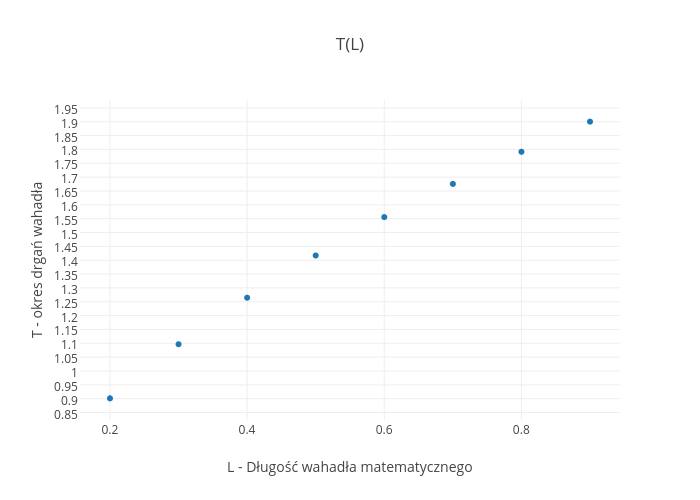
\includegraphics[height=0.5\textheight]{Plot2.png}\\
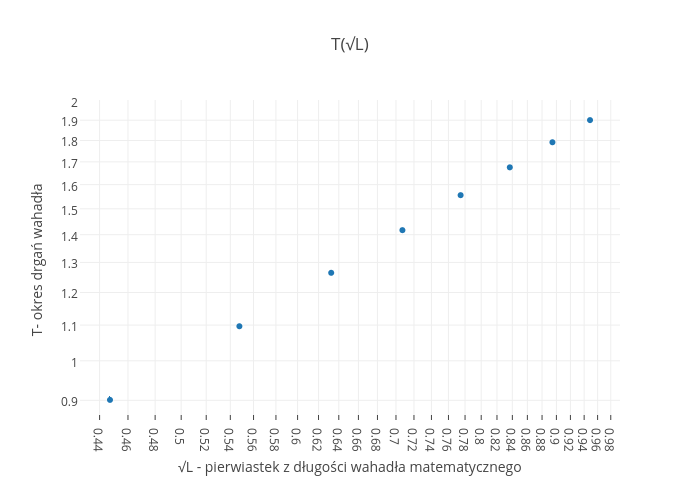
\includegraphics[height=0.5\textheight]{Plot5.png}\\
Słupki niepewności są tak małe, że na wykresie są niewidoczne.\\\\\\
Metodą regresji liniowej wyznaczyliśmy współczynniki prostej $T(\sqrt{L})$, które wynoszą:                      
wyraz wolny 
$$a = 0,010586$$
oraz współczynnik regresji 
$$b = 1,99101093$$
co w rezultacie daje nam równanie prostej
$$y=bx + a$$
$$y=1,99101093x + 0,010586$$
Stąd niepewności współczynników wynoszą kolejno 
$$u(a) = 0,0061118$$
oraz 
$$u(b) = 0,021154$$
Opierając się na współczynniku $b$ oraz równaniu ruchu możemy obliczyć przyspieszenie ziemskie $$g = \frac{4\pi^2}{1,99101093} = 9,868468842 \frac{m}{s^2}$$
następnie w oparciu o prawo przenoszenia niepewności, obliczamy niepewność wyznaczonej wartości $u(g)$ ze wzoru:
$$u(g) = \sqrt{(\frac{4\pi^2}{a^2} \cdot u(a))^2}$$
więc, $u(g) = 0,0045132$.\\
Niepewność rozszerzoną obliczamy ze wzoru:
$$U(g)=k_p \cdot u(g)$$
, gdzie $k_p$ to współczynnik rozszerzenia równy $2$.
$$U(g)=2\cdot u(g)=2\cdot 0,0045132=0,0090264s$$\\



Aby obliczyć przyspieszenie ziemskie dla szerokości geograficznej oraz wysokości nad poziomem morza Gliwic potrzebowaliśmy danych, które wynoszą $h=240 m.n.p.m.$ oraz $\varphi = 50,31^{\circ}$. Podstawiając wartości do wzoru:
$$g\approx 9780318(1+0,0053024\sin^2 \varphi-0,0000058\sin^2 2\varphi ) - 3,086\cdot 10^{-6}h \approx 9,7796 \frac{m}{s^2}$$
\subsection{Test zgodności}
Dla otrzymanych wartości, test zgodności przeprowadzamy przy pomocy wzoru:
$$\frac{|x-y|}{\sqrt{u^2(x) + u^2(y)}} \approx 5,28$$
gdzie y to wartość przyspieszenia ziemskiego tablicowa, a x to obliczona wartość $g$.
\subsection{Wnioski}
Okres wahnięć wahadła jest zależy od jego długości. Otrzymane wyniki odbiegają od siebie o około $0,1\frac{m}{s^2}$, więc można określić je jako zbliżone. Powodem niezgodności może być zbyt duże odchylenie wahadła podczas pomiarów.

\end{document}